\documentclass[12pt]{article}

\usepackage{graphicx}
\usepackage{paralist}
\usepackage{amsfonts}
\usepackage{hyperref}
\usepackage{listings}
\usepackage{subfig}
\usepackage{float}

\oddsidemargin 0mm
\evensidemargin 0mm
\textwidth 160mm
\textheight 200mm
\renewcommand\baselinestretch{1.0}

\pagestyle {plain}
\pagenumbering{arabic}
\newcounter{stepnum}

\title{Course Project}
% \author{Hyosik Moon}
\author{
  Moon, Hyosik
  }

\begin {document}

\maketitle

\section{Required}

\begin{itemize}
\item \textbf{Main objective of the analysis} \\
I will analyze the Goldman Sachs's Stock Data from 1999-05-04 to 2021-07-01 with time series models such as RNN and LSTM.

\item \textbf{Brief description of the data set} \\
In the data, there are seven features such as `Date, Open, High, Low, Close, Adj Close, and Volume' (Figure \ref{data}). We will use `Date' and `Close' features to predict stock price. To be specific, we will train models with for about past 20 years data and predict the upcoming 7 months' Goldman Sachs's stock price.

\begin{figure}[H]
  \centering
  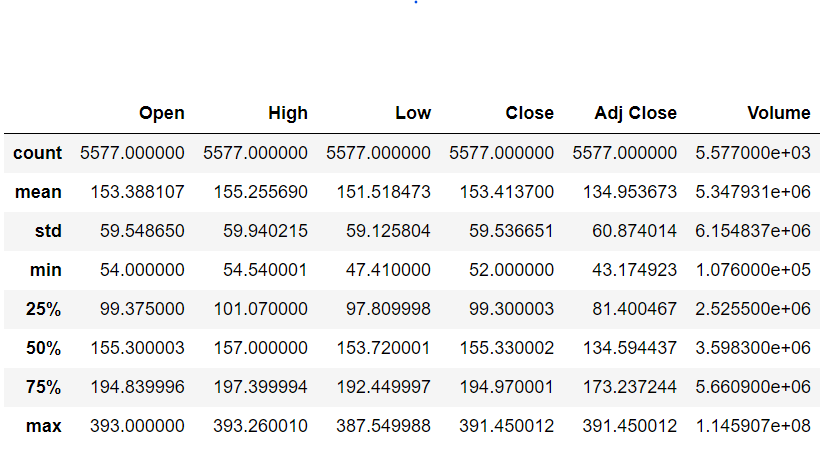
\includegraphics[width=0.9\textwidth]{figures/data.png}
  \caption{Data description without date}\label{data}
\end{figure}

\item \textbf{Brief summary of data exploration}
I remained only `Data', and `Close' features. In order to use for RNNs and LSTMs it needs a 3D numpy array of shape (n\_sample, time\_steps, n\_features). As I learned in the class I made a function to preprocess train\_test data sets. And I train the RNN models with `cell\_units = 30, epochs = 100, loss=mean\_squared\_error, optimizer=adam'.

\item \textbf{Summary of training at least three models} I implemented the data with `RNN, LSTM' models.
    \begin{enumerate}
      \item Recurren Neural Networks. I trained RNNs with 5577 days' data and predicted following 420 days. As you expected the result was very poor. It was an obvious result becuase RNN's prediction accuracy is very bad for long-term period. (Figure \ref{rnn})
      \begin{figure}[H]
        \centering
        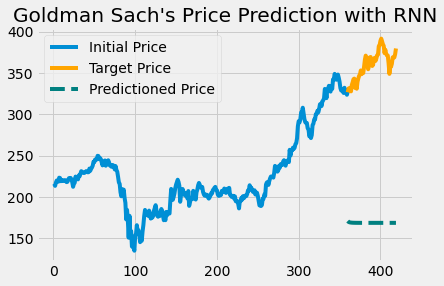
\includegraphics[width=0.9\textwidth]{figures/rnn.png}
        \caption{Recurrent Neural Networks}\label{rnn}
      \end{figure}

      \item LSTM. Unfortunately the result was also bad (Figure \ref{lstm}).
      \begin{figure}[H]
        \centering
        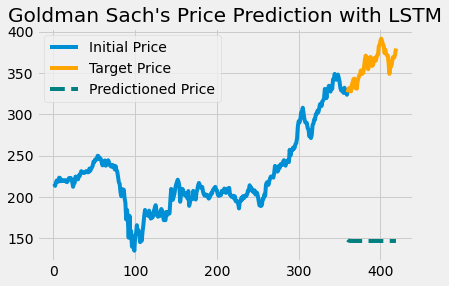
\includegraphics[width=0.9\textwidth]{figures/lstm.png}
        \caption{Long Short Term Memory}\label{lstm}
      \end{figure}
    \end{enumerate}
\item \textbf{Explanation of your final model}
I needed to analyze the result. When I inspected the codes, it seemed not to have an error. Thus, I modified the length of data from (5577, 360, 1) to (1260, 210, 1) and epochs from 300 to 1200. Interestingly RNNs also showed much better result even I trained the model with fewer data (Figure \ref{rnn2}). However, for LSTM it showed still bad predction accuracy (Figure \ref{lstm2}). So, I trained more but with short date, i.e. from [data = (1260, 210, 1), nodes = 30, epochs = 1200] to [data = (1260, 210, 1), nodes = 70, epochs=1400] (Figure \ref{lstm3}). Because it still shows bad result, I added more nodes to 100 and trained again (Figure \ref{lstm4}). It looks a little bit better but still quite bad. When I see the trained result the prediction error was low, so I thought that the reason of low accuracy maybe is for the number of nodes not the epochs. So I inceased the number of nodes from 100 to 210 which is same number of the time\_steps and decrease the epochs from 1200 to 1000 to reduce the training time. It shows still bad result.. So I changed the length of training data from 1260 to 2000 and decrease the epochs to 350 (Figure \ref{lstm6}). As the result of 7 analysis, all models seem not to be appropriate to predict the stock price. However the last one (LSTM6) shows a liitle bit better predction result compared to the others. 


\begin{figure}[H]
  \centering
  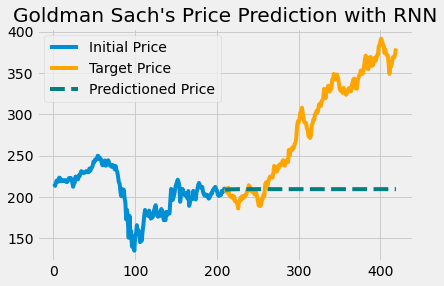
\includegraphics[width=0.9\textwidth]{figures/rnn2.png}
  \caption{RNN with data = (630, 210, 1), nodes = 30, epochs = 1200}\label{rnn2}
\end{figure}

\begin{figure}[H]
  \centering
  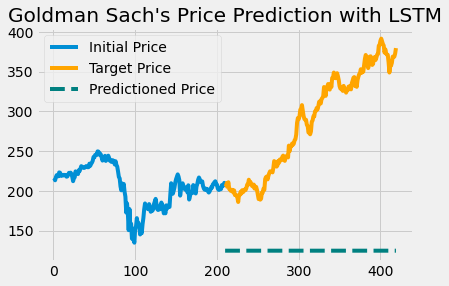
\includegraphics[width=0.9\textwidth]{figures/lstm2.png}
  \caption{Long Short Term Memory2 = (1260, 210, 1), nodes = 30, epochs = 1200}\label{lstm2}
\end{figure}

\begin{figure}[H]
  \centering
  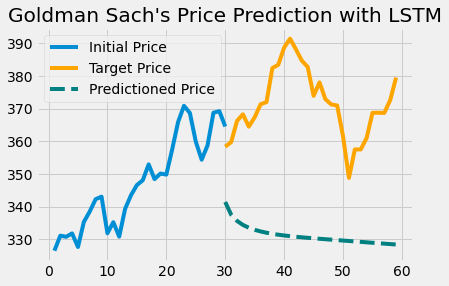
\includegraphics[width=0.9\textwidth]{figures/lstm3.png}
  \caption{Long Short Term Memory3 = (1260, 210, 1), nodes = 70, epochs = 1400}\label{lstm3}
\end{figure}

\begin{figure}[H]
  \centering
  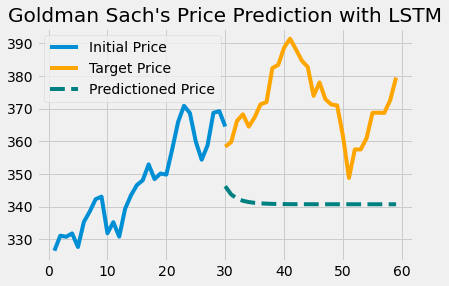
\includegraphics[width=0.9\textwidth]{figures/lstm4.png}
  \caption{Long Short Term Memory4 = (1260, 210, 1), nodes = 100, epochs = 1200}\label{lstm4}
\end{figure}

\begin{figure}[H]
  \centering
  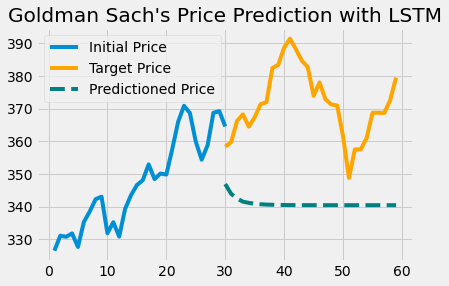
\includegraphics[width=0.9\textwidth]{figures/lstm5.png}
  \caption{Long Short Term Memory5 = (1260, 210, 1), nodes = 210, epochs = 1000}\label{lstm5}
\end{figure}

\begin{figure}[H]
  \centering
  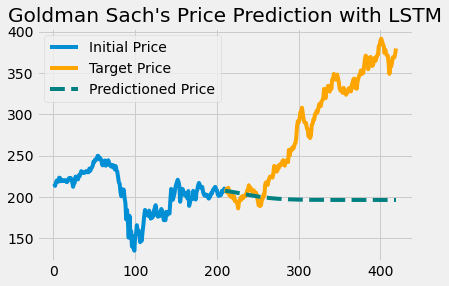
\includegraphics[width=0.9\textwidth]{figures/lstm6.png}
  \caption{Long Short Term Memory6 = (2000, 210, 1), nodes = 210, epochs = 350}\label{lstm6}
\end{figure}



\item \textbf{Summary Key Findings and Insights}
In the real world, most of data are non-stationary data. So, we need to manipulate the data to stationary data by subtracting trends and seasonality. Then the data should show constant mean and variance, which is a very picky condition. Thus, it needs expertise to analyze and manipulate the data correctly. However, in the case of Deep Learning Models for time series analysis such as RNNs and LSTM, doesn't need to manipulate data to make stationary. It's really incredible fact because even if not an expert can predict the time series data if they have a little knowledge and skills about deep learning. I think it's the magic of the deep learning. But in order to gurantee the accuracy of the model and interpretation of the models we need deep theoroetical knowledge, high comuputing power, and huge amount of data. If not, as we've seen in this report, we can't gurantee the reliability of the model and the result.


\item \textbf{Suggestions for next steps}
In oder to predict the stock price more accurately, I think using the ground truth values seems to be more appropriate rather than predicting following values with previously predicted values (Figure \ref{lstm7}). In the figure (LSTM7) we can see that after 300 days the model seems to stop to predict. There seems to be an error in the model.. We need to analyze the reason of it. And I was sorry that I wasn't able to use Facebook Prophet models to predict the time series data. It had a problem to install, and I wasn't able to figure it out. If I can solve the installing issure, I'd like to use Facebook Prophet libraries for the time series analysis.

\begin{figure}[H]
  \centering
  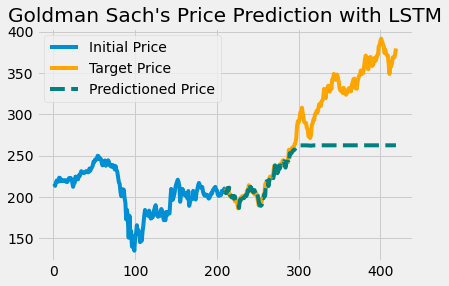
\includegraphics[width=0.9\textwidth]{figures/lstm7.png}
  \caption{Long Short Term Memory7 = (2000, 210, 1), nodes = 210, epochs = 350}\label{lstm7}
\end{figure}

\end{itemize}

\end{document}